\documentclass[oneside,listof=totoc]{scrbook}

% PENGATURAN
% Pengaturan ukuran kertas dan margin
\usepackage{geometry}
\geometry{
  a4paper,
  lmargin=40mm,
  rmargin=30mm,
  tmargin=40mm,
  bmargin=30mm
}
\usepackage{rotating}

% Pengaturan jarak antar baris
\usepackage{setspace}
\linespread{1.5}
\newcommand\tab[1][1cm]{\hspace*{#1}}

% Pengaturan font
\usepackage{fontspec}
\setmainfont{Times New Roman}

% Pengaturan daftar isi, daftar gambar, daftar tabel, daftar pustaka
\usepackage{hyperref}
\hypersetup{
    colorlinks=true,
    linkcolor=black,
    filecolor=black,
    urlcolor=blue,
}
\usepackage{hanging}
\setuptoc{toc}{totoc}
\usepackage[titles]{tocloft}
\setlength{\cftchapnumwidth}{42pt}
\setlength{\cftsecnumwidth}{27pt}
\setlength{\cfttabnumwidth}{49pt}
\setlength{\cftfignumwidth}{62pt}
\renewcommand{\cftchappresnum}{\chaptername\ }
\renewcommand{\cftchapdotsep}{\cftdotsep}
\renewcommand{\cftchapfont}{\normalfont\bfseries}
\renewcommand{\cfttabpresnum}{\tablename\ }
\renewcommand{\cfttabfont}{\normalfont\bfseries}
\renewcommand{\cftfigpresnum}{\figurename\ }
\renewcommand{\cftfigfont}{\normalfont\bfseries}
\renewcommand{\contentsname}{DAFTAR ISI}
\renewcommand{\listfigurename}{DAFTAR GAMBAR}
\renewcommand{\listtablename}{DAFTAR TABEL}

% Pengaturan gambar, label, caption, dan items
\usepackage{enumitem}
\usepackage{pgf,tikz}
\usepackage{caption}
\captionsetup[figure]{labelsep=space}
\renewcommand{\thefigure}{\arabic{chapter}.\arabic{figure}}
\renewcommand{\figurename}{\bfseries{Gambar}}
\renewcommand{\tablename}{\bfseries{Tabel}}
\renewcommand{\labelitemi}{\bfseries{--}}

% Pengaturan tabel
\captionsetup[table]{labelsep=space}
\renewcommand{\thetable}{\arabic{chapter}.\arabic{table}}
\usepackage{color, colortbl}
\definecolor{Gray}{gray}{0.7}
\usepackage{array}
\newcolumntype{x}[1]{>{\raggedright\arraybackslash}p{#1}}
\usepackage{multirow}

% Pengaturan rumus matematika
\usepackage{amsmath}

% Pengaturan bab dan subbab
\renewcommand{\chaptername}{BAB}
\renewcommand{\thechapter}{\Roman{chapter}}
\renewcommand{\thesection}{\arabic{chapter}.\arabic{section}}
\renewcommand{\thesubsection}{\arabic{chapter}.\arabic{section}.\arabic{subsection}}
\renewcommand{\thesubsubsection}{\arabic{chapter}.\arabic{section}.\arabic{subsection}.\arabic{subsubsection}}
\renewcommand{\theequation}{\arabic{chapter}.\arabic{equation}}

\usepackage{titlesec}
\titleformat{\chapter}[display]
  {\normalsize\bfseries\centering}{\chaptertitlename\ \thechapter}{0pt}{}
  \titlespacing*{\chapter}{0pt}{-\topskip}{0pt}
\titleformat{\section}
  {\normalsize\bfseries}{\thesection}{12pt}{}
\titleformat{\subsection}
  {\normalsize\bfseries}{\thesubsection}{12pt}{}
\titleformat{\subsubsection}
  {\normalsize\bfseries}{\thesubsubsection}{12pt}{}
\titleformat{\paragraph}
  {\normalsize\bfseries}{\theparagraph}{12pt}{}
\usepackage{indentfirst}
\setlength{\parindent}{25pt}

\RedeclareSectionCommand[
  afterskip=1.5ex plus .2ex,
  beforeskip=-3.25ex plus -1ex minus -.2ex
]{paragraph}
\setcounter{secnumdepth}{\paragraphnumdepth}
\setcounter{tocdepth}{\paragraphtocdepth}

% Pengaturan nomor halaman (konfigurasi pada masing-masing matter)
\usepackage{fancyhdr}

% Global variabel (tahun, nama, nim, dll)
\newcommand{\JudulProposal}{JUDUL SKRIPSI DALAM BAHASA INDONESIA \\ DITULIS SECARA SIMETRIS}
\newcommand{\NamaMahasiswa}{Nama Mahasiswa}
\newcommand{\NIM}{12.34.567}
\newcommand{\DosenPembimbingUtama}{Dosen Pembimbing Utama}
\newcommand{\NIDNDosenPembimbingUtama}{NIDN 1234567890}
\newcommand{\DosenPembimbingPendamping}{Dosen Pembimbing Pendamping}
\newcommand{\NIDNDosenPembimbingPendamping}{NIDN 1234567890}
\newcommand{\TanggalPembuatan}{00}
\newcommand{\BulanPembuatan}{Bulan}
\newcommand{\TahunPembuatan}{2020}

\begin{document}

% FRONT MATTER
\frontmatter
\pagestyle{plain}

% Halaman: JUDUL
\clearpage
\thispagestyle{empty}

\begin{center}
  \normalsize{\textbf{PROPOSAL SKRIPSI}\\
  \vspace{1.0cm}
  \textbf{\JudulProposal}}\\
  \textbf{(Studi Kasus: Tempat Penelitian Skripsi-jika ada, opsional)}
\end{center}

\vspace{3.0cm}

\begin{minipage}{12.2cm}
  \centering
    
\includegraphics[width=4.20cm]{gambar/logo_um}
\end{minipage}

\vspace{2.5cm}

\begin{center}
  \normalsize{Disusun oleh:}\\
  \vspace{0.2cm}
  \begin{minipage}{\textwidth}
    \begin{center}
      \begin{tabular}{l r l}
        \textbf{Nama} & : & \textbf{\NamaMahasiswa}\\
        \textbf{NIM}  & : & \textbf{\NIM}
      \end{tabular}
    \end{center}
  \end{minipage}
\end{center}

\vspace{3.0cm}

\begin{center}
  \normalsize{\textbf{PROGRAM STUDI INFORMATIKA-S1}}\\
  \normalsize{\textbf{FAKULTAS ILMU KOMPUTER}}\\
  \normalsize{\textbf{UNIVERSITA MULIA}}\\
  \normalsize{\textbf{BALIKPAPAN}}\\
  \normalsize{\textbf{\TahunPembuatan}}
\end{center}

% Halaman: HALAMAN PERSETUJUAN
\chapter{HALAMAN PERSETUJUAN}

\vspace{1.0cm}

\begin{center}
  \normalsize{\textbf{\JudulProposal}}
\end{center}

\vspace{3.0cm}

\begin{center}
  \normalsize{Dipersiapkan dan Disusun oleh}\\
  \textbf{\NamaMahasiswa}\\
  \textbf{\NIM}
\end{center}

\vspace{3.0cm}

\begin{center}
  \linespread{1.0}
  \normalsize{Telah disetujui oleh Tim Dosen Pembimbing Skripsi\\
  pada tanggal, \TanggalPembuatan\ \BulanPembuatan\ \TahunPembuatan}
\end{center}

\vspace{3.0cm}

\begin{minipage}{\textwidth}
  \tab[0cm]\textbf{Pembimbing Utama} \tab[4.5cm] \textbf{Pembimbing Pendamping}\\
  \vspace{1.3cm}\\
  \linespread{1.0}
  \normalsize{\tab[0cm]\textbf{\underline{\DosenPembimbingUtama}} \tab[3.4cm] \textbf{\underline{\DosenPembimbingPendamping}}\\
  \tab[0cm]\textbf{\NIDNDosenPembimbingUtama} \tab[4.80cm] \textbf{\NIDNDosenPembimbingPendamping}}
\end{minipage}

% Halaman: DAFTAR ISI, DAFTAR TABEL, DAFTAR GAMBAR
\tableofcontents
\listoftables
\listoffigures

% MAIN MATTER
\mainmatter
\pagestyle{fancy}\fancyhf{}\fancyhead[R]{\thepage}
\renewcommand{\headrulewidth}{0pt}

% Halaman: BAB I
\chapter{PENDAHULUAN}

\vspace{0.5cm}

\section{Latar Belakang}
Bagian ini memuat penjelasan tentang fenomena umum yang terjadi dan kemudian dipersempit mengarah ke permasalahan yang akan diteliti/dibahas. Latar belakang masalah merupakan uraian yang komprehensif mengenai pentingnya permasalahan tersebut diangkat menjadi topik penelitian ditinjau dari aspek praktis maupun kontribusi ilmiah secara teoritis.

Penulisan latar belakang masalah disajikan dalam bentuk uraian yang secara kronologis diarahkan untuk langsung menuju rumusan masalah.

Dalam latar belakang masalah dimasukkan beberapa uraian permasalahan yang terjadi, yang dapat memperkuat alasan atau motivasi mengapa perlu diadakan penelitian seperti yang mahasiswa ajukan.

\section{Rumusan Masalah}
Bagian ini memuat penjelasan tentang permasalahan sehingga memerlukan solusi penelitian. Permasalahan yang diuraikan dalam latar belakang masalah dirumuskan kembali secara tegas dan jelas dalam bentuk poin-poin yang terinci yang berisi masalah-masalah yang akan dikaji pada penelitian.

\noindent Contoh:

\noindent Berdasarkan latar belakang masalah di atas, maka permasalahan yang akan dibahas/diteliti dalam Skripsi ini dirumuskan sebagai berikut:

\begin{enumerate}[label=\alph*.]
  \item Bagaimana............?
  \item Bagaimana............?
\end{enumerate}

\section{Batasan Masalah}
Bagian ini memuat penjelasan tentang :

\begin{enumerate}[label=\alph*.]
  \item Batasan-batasan permasalahan yang akan dicari solusinya dengan penelitian yang akan dilakukan.
  \item Asumsi-asumsi yang digunakan sebagai dasar untuk melaksanakan penelitian.
  \item Batasan solusi yang dilakukan pada penelitian.
\end{enumerate}

\section{Tujuan Penelitian}
Bagian ini memuat penjelasan secara spesifik:

\begin{enumerate}[label=\alph*.]
  \item Solusi yang ditawarkan untuk menangani permasalahan yang dihadapi
  \item Hal-hal yang ingin dicapai melalui kegiatan penelitian yang akan dilakukan.
  \item Sebagai salah satu syarat kelulusan pada Program Studi Informatika Fakultas Ilmu Komputer Universitas Mulia Balikpapan.
  \item Tujuan tersebut harus dikaitkan langsung dengan judul dan latar belakang masalah
\end{enumerate}

\section{Manfaat Penelitian}
Bagian ini memuat penjelasan tentang:

\begin{enumerate}[label=\alph*.]
  \item Manfaat/kontribusi ilmiah dalam ilmu pengetahuan jika penelitian tersebut berhasil.
  \item Kegunaan atau kemampuan dari sistem yang akan diteliti jika penelitian tersebut berhasil.
  \item Manfaat yang dapat dirasakan oleh perusahaan/pemakai apabila hasil penelitian tersebut diterapkan di perusahaan.
\end{enumerate}

% Halaman: BAB II
\chapter{LANDASAN TEORI}

\vspace{0.5cm}

\section{Tinjauan Pustaka}
Tinjauan Pustaka merupakan sarana untuk menunjukkan keaslian penelitian. Bagian ini memuat uraian sistematis tentang informasi hasil penelitian sebelumnya, minimal 5 buah, yang relevan dengan penelitian yang akan dilakukan. Penelitian yang dijadikan rujukan paling lama selisih 3 tahun dari penelitian yang akan dilakukan, diambil dari publikasi ilmiah yang berkualitas, serta memuat kelebihan dan kelemahan masing-masing.

Bagian ini juga memuat penegasan posisi penelitian yang dilakukan oleh mahasiswa terhadap penelitian-penelitian sebelumnya dan relevansinya dengan masalah penelitian yang sedang diteliti. Fakta-fakta yang dikemukakan sejauh mungkin diacu dari sumber asli. Referensi tidak dari sumber aslinya hanya boleh dilakukan dalam keadaan terpaksa (sumber asli sangat sulit ditemukan).

Selain itu, bagian ini berisi justifikasi atau kritik pada kelemahan atau kekurangan yang mungkin ada pada penelitian terdahulu sehingga dapat dijadikan argumen bahwa penelitian yang akan dilakukan bersifat penyempurnaan atau pengembangan penelitian terdahulu. Sumber pustaka yang dirujuk pada bagian ini harus dicantumkan dalam kalimat atau pernyataan yang diacu dan dicantumkan dalam daftar pustaka.

\clearpage
\begin{sidewaystable}
\vspace{-2.5cm}
\section{Keaslian Penelitian}

\noindent\begin{minipage}{\textwidth}
  \label{tabel:2.1}
  \captionof{table}{\bfseries{Matriks Literatur Review dan Posisi Penelitian}}
  \centering\bfseries{\JudulProposal}\\
  \vspace{0.5cm}
  \setstretch{1.0}
  \normalfont
  \setlength\extrarowheight{2pt}
  \begin{tabular}{|c|p{3.0cm}|p{2.5cm}|p{3.0cm}|p{3.0cm}|p{4.0cm}|p{4.5cm}|}
    \hline
    \cellcolor{Gray}\textbf{No.} & \multicolumn{1}{m{3.0cm}|}{\cellcolor{Gray}\centering\textbf{Judul}} & \multicolumn{1}{m{2.5cm}|}{\cellcolor{Gray}\centering\textbf{Peneliti, Media Publikasi, dan Tahun}} & \multicolumn{1}{m{3.0cm}|}{\cellcolor{Gray}\centering\textbf{Tujuan Penelitian}} & \multicolumn{1}{m{3.0cm}|}{\cellcolor{Gray}\centering\textbf{Kesimpulan}} & \multicolumn{1}{m{4.0cm}|}{\cellcolor{Gray}\centering\textbf{Saran atau Kelemahan}} & \multicolumn{1}{m{4.5cm}|}{\cellcolor{Gray}\centering\textbf{Perbandingan}}\\
    \hline
    1. & Judul Penelitian & \raggedright Nama peneliti, media publikasi, tahun penelitian & \raggedright Apa tujuan penelitian tersebut? & \raggedright Apa kesimpulan penelitian tersebut? Kesimpulan harus menjawab rumusan masalah & \raggedright Apa saran penelitian selanjutnya, atau apa kelemahan utama pada penelitian tersebut? & \raggedright Perbedaan antara hasil penelitian sebelumnya dengan penelitian yang akan dilakukan, diantaranya berkaitan dengan metode yang digunakan, inovasi, serta kompleksitas permasalahan yang diajukan sehingga perbedaan tidak sekedar pada objek penelitian.\tabularnewline
    \hline
    2. & Minimal 5 Penelitian terbaru & & & & & \\
    \hline
  \end{tabular}
\end{minipage}
\end{sidewaystable}

\clearpage
\section{Teori-Teori yang Digunakan}
Bagian ini memuat rangkuman teori-teori yang diambil dari buku atau literatur yang mendukung penelitian, serta memuat penjelasan tentang konsep dan prinsip dasar yang diperlukan untuk pemecahan permasalahan. Landasan teori dapat berbentuk uraian kualitatif, model matematis, atau tools yang langsung berkaitan dengan permasalahan yang diteliti. Sumber teori yang dirujuk pada bagian ini harus dicantumkan dalam kalimat atau pernyataan yang diacu dan dicantumkan dalam Daftar Pustaka.

\subsection{Judul Sub 2.3.1 Teori-Teori yang Digunakan}
Judul ini merupakan bagian dari sub judul 2.3.1 dari sub judul Landasan Teori...

\subsection{Judul Sub 2.3.2 Teori-Teori yang Digunakan}
Judul ini merupakan bagian dari sub judul 2.3.2 dari sub judul Landasan Teori...

\noindent Contoh Gambar.

\vspace{0.5cm}

\begin{center}
  \begin{minipage}{\textwidth}
    \label{gambar:2.1}
    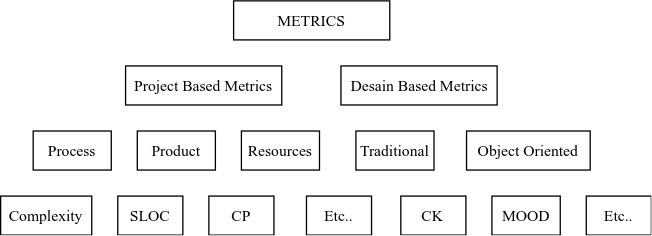
\includegraphics[width=13.5cm]{gambar/gambar_2.1.png}
    \vspace{0.5cm}
    \captionof{figure}{\bfseries{Judul Gambar Posisi di Bawah Gambar Cetak Tebal}}
  \end{minipage}
\end{center}

\clearpage
\subsubsection{Judul Sub 2.3.2.1 Landasan Teori}
Judul ini merupakan bagian dari sub judul 2.3.2.1 dari sub judul Landasan Teori...

\vspace{0.5cm}

\noindent\begin{minipage}{\textwidth}
  \label{tabel:2.2}
  \captionof{table}{\bfseries{Judul Tabel 2.2 Posisi di Atas Tabel Rata Tengah Cetak Tebal}}
  \setstretch{1.0}
  \normalfont
  \setlength\extrarowheight{2pt}
  \vspace{0.5cm}
  \hspace{1.1cm}
  \begin{tabular}{|c|l|c|}
    \hline
    \rowcolor{Gray}
    Source & \multicolumn{1}{c|}{\cellcolor{Gray}Metrics} & OO Construct \\ \hline
    & Cyclomatic Complexity (CC) &  \\ \cline{2-2}
    & Lines Of Code (LOC) &  \\ \cline{2-2}
    \multirow{-3}{*}{Traditional Metrics} & Comment Percentage (CP) & \multirow{-3}{*}{Method} \\ \hline
    & \begin{tabular}[c]{@{}l@{}}Weighted Method Per Class\\ (WMC)\end{tabular} & Class/Method \\ \cline{2-3}
    & Response For Class (RFC) & Class/Message \\ \cline{2-3}
    & \begin{tabular}[c]{@{}l@{}}Lack of Cohesion Of Methods\\ (LCOM)\end{tabular} & Class/Cohesion \\ \cline{2-3}
    & \begin{tabular}[c]{@{}l@{}}Coupling Between Objects\\ (CBO)\end{tabular} & Coupling \\ \cline{2-3}
    & \begin{tabular}[c]{@{}l@{}}Depth of Inheritance Tree\\ (DIT)\end{tabular} & Inheritance \\ \cline{2-3}
    \multirow{-6}{*}{New Object Oriented} & Number Of Children (NOC) & Inheritance \\ \hline
  \end{tabular}
\end{minipage}

\vspace{0.5cm}

\paragraph{\normalfont\bfseries{Judul Sub 2.3.2.1.1 Teori-Teori yang Digunakan}}
Judul ini merupakan bagian dari sub judul 2.2.2.1.1 dari sub judul Landasan Teori...

\subsection{Judul Sub 2.3.3 Teori-Teori yang Digunakan}
Judul ini merupakan bagian dari sub judul 2.3.3 dari sub judul Landasan Teori...

\vspace{0.5cm}

\begin{center}
  \begin{minipage}{\textwidth}
    \label{gambar:2.2}
    \hspace{1.8cm}
    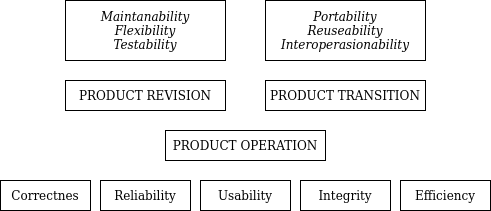
\includegraphics[width=10.5cm]{gambar/gambar_2.2.png}
    \vspace{0.5cm}
    \captionof{figure}{\bfseries{Judul Gambar 2 Posisi di Bawah Gambar Cetak Tebal Tanpa Titik}}
  \end{minipage}
\end{center}

\vspace{0.5cm}

\noindent\begin{minipage}{\textwidth}
  \label{tabel:2.3}
  \captionof{table}{\bfseries{Judul Tabel 2.3 Posisi di Atas Tabel Rata Tengah Cetak Tebal Tanpa Titik}}
  \setstretch{1.0}
  \normalfont
  \setlength\extrarowheight{2pt}
  \vspace{0.5cm}
  \hspace{-0.2cm}
  \begin{tabular}{|l|l|l|}
    \hline
    \rowcolor{Gray}
    \multicolumn{1}{|c|}{\cellcolor{Gray}} & \multicolumn{2}{c|}{\cellcolor{Gray}\textbf{Parameter Metrik}} \\ \cline{2-3}
    \rowcolor{Gray}
    \multicolumn{1}{|c|}{\multirow{-2}{*}{\cellcolor{Gray}\textbf{Faktor-faktor Kualitas Software}}} & \multicolumn{1}{c|}{\cellcolor{Gray}\textbf{Traditional Metrics}} & \multicolumn{1}{c|}{\cellcolor{Gray}\textbf{CK Metrics Suite}} \\ \hline
    \textit{efficiency} & - & LCOM,CBO,DIT,NOC \\ \hline
    \textit{complexity} & CC & - \\ \hline
    \textit{understandability} & CP,LOC & WMC,RFC,DIT \\ \hline
    \textit{reusability} & CP,LOC & WMC,LCOM,CBO,DIT,NOC \\ \hline
    \textit{maintainability/testability} & CP,LOC & WMC,RFC,DIT,NOC \\ \hline
  \end{tabular}
\end{minipage}

\vspace{0.5cm}

\noindent Contoh penulisan Rumus Matematika :

\begin{equation}
Mi = \prod_{j=1}^n bij,i=1,2,...,n
\end{equation}

\begin{enumerate}
\item Menghitung n akar pangkat dari \textit{Mi}
  \begin{equation}
  \overline{W}i = \sqrt[n]{Mi}
  \end{equation}

\item Melakukan normalisasi terhadap $ \overline{W}i $
  \begin{equation}
  Wi = \overline{W}i / \Sigma_{j=1}^n \overline{W}i,i = 1,2,...,n
  \end{equation}

\item Mencari Lamda maksimal adalah :
  \begin{equation}
  \lambda maks = \Sigma_{i=1}^n \Sigma_{j=1}^n bijWj
  \end{equation}
\end{enumerate}

% Halaman: BAB III
\chapter{METODOLOGI PENELITIAN}

\vspace{0.5cm}

\section{Metode Penelitian}
Bagian ini memuat penjelasan secara lengkap dan terinci tentang langkah-langkah yang dilakukan dalam melakukan penelitian dimulai dari perumusan permasalahan hingga pengambilan kesimpulan. Selain itu, langkah penelitian juga perlu ditunjukkan dalam bentuk diagram alir langkah penelitian atau framework secara lengkap dan terinci termasuk di dalamnya tercermin algoritma, rule, pemodelan-pemodelan, desain dan lain-lain yang terkait dengan aspek perancangan sistem.

\section{Metode Pengumpulan Data}
Bagian ini memuat penjelasan secara lengkap dan terinci tentang cara-cara yang digunakan dalam proses pengumpulan data untuk jenis data yang diperlukan. Misalnya melalui observasi, wawancara, eksperimen, atau penyebaran angket. Jika metode penyebaran angket digunakan, maka blangko angket harus dilampirkan dalam Skripsi. Untuk setiap metode pengumpulan data, harus dijelaskan tentang jenis data yang dikumpulkan dengan metode-metode yang terkait. Bagian ini juga memuat penjelasan secara lengkap dan terinci tentang jenis data yang diperlukan untuk analisis dalam pembahasan.

\section{Metode Analisis Data}
Bagian ini memuat penjelasan secara lengkap dan terinci tentang metode dan alat yang digunakan untuk analisis data.

\noindent Catatan:

Dalam hal penelitian berupa rekayasa atau desain, maka penjelasan pada bagian ini dapat disesuaikan dengan permasalahannya. Dengan alasan untuk penyempurnaan atau perbaikan, maka Dosen Pembimbing Utama dan Dosen Pembimbing Pendamping berhak untuk memberikan revisi terhadap Skripsi.

\section{Metode Pengembangan Proses Perangkat Lunak (Optional)}
Bagian ini memuat tentang model proses pengembangan perangkat lunak yang digunakan dalam penelitian misalnya menggunakan Waterfall / SDLC / Incremental dll.

\section{Metode Perancangan (Optional)}
Jika membuat aplikasi komputer: menggunakan model flowchart untuk menggambarkan proses yang diusulkan, atau menggunakan model normalisasi data untuk mendapatkan struktur tabel data yang ideal, atau model DFD hingga gambaran Relasi Antar Tabel, atau melakukan perancangan dengan model ERD, UML dengan Diagram Activity, Metode USDP (Unified Software Development Process), dll.

\section{Metode Testing (Optional)}

\subsection{White-box Testing (menggunakan Software Testing Standard)}
Dalam uji coba program ada beberapa cara pengujian, diantaranya pengujian kesalahan sintaks, kesalahan logika. Menurut Pressman, ada 2 jenis pengujian system yaitu: white-box testing dan black-box testing. Jelaskan tahapan-tahapan bagaimana melakukan pengujian terhadap sistem dan program yang sudah dibuat sehingga system tersebut bebas dari kesalahan (bugs) dan dapat dilanjutkan ke proses selanjutnya, yaitu: proses implementasi sistem ke perusahaan / objek penelitian. Disarankan untuk menggunakan software yang sudah terstandar dan di akui untuk menguji listing program yang sudah dibuat.

\subsection{Black-box Testing}
Pengujian pemakaian aplikasi oleh user, untuk mengetahui apakah aplikasi sudah benar-benar siap digunakan, testing menu-menu dan fungsi yang ada, apakah sudah sesuai dengan kebutuhan dan bentuk laporan sudah sesuai keinginan user.

\clearpage
\section{Alur Penelitian}
Contoh Alur Penelitian :

\vspace{0.5cm}

\begin{center}
  \begin{minipage}{\textwidth}
    \label{gambar:3.1}
    \hspace{1.8cm}
    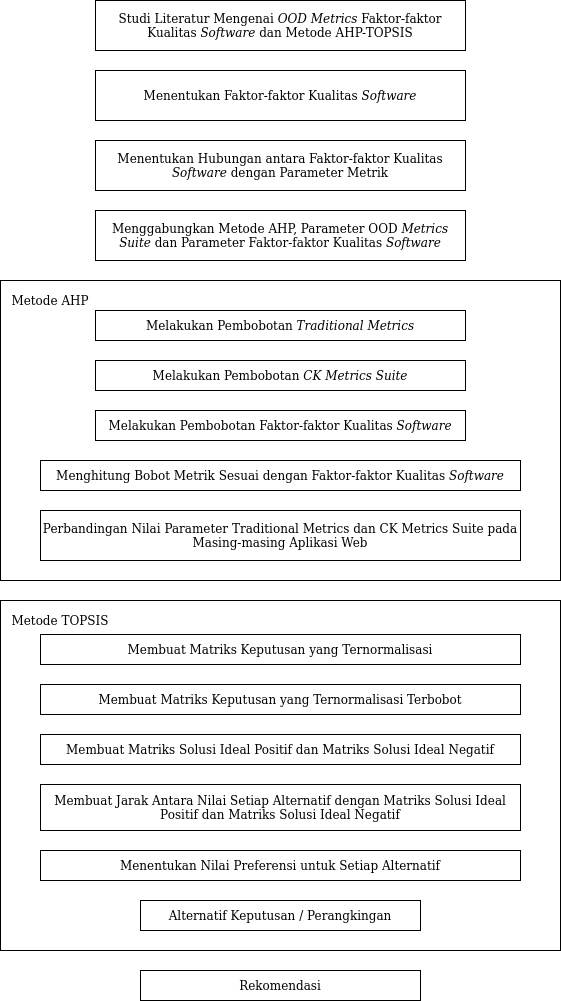
\includegraphics[width=10.5cm]{gambar/gambar_3.1.png}
    \vspace{0.5cm}
    \captionof{figure}{\bfseries{Alur Penelitian}}
  \end{minipage}
\end{center}


% BACK MATTER
\backmatter
\pagestyle{plain}

% Halaman: DAFTAR PUSTAKA
\chapter{DAFTAR PUSTAKA}

\vspace{0.5cm}

\begin{singlespace}
\noindent\textbf{PUSTAKA BUKU}\\

\begin{hangparas}{25pt}{1}
Nama pengarang, tahun penerbitan, judul, edisi (jika perlu), jilid (jika perlu), nama penerbit, kota penerbit.\\

Pressman, R. S., 2010, \textit{Software Engineering A Practitioner’s Approach}, Seventh Edition, McGraw Hill, New York.\\

Pressman, R. S.; Lowe,D., 2009, \textit{Web Engineering A Practitioner’s Approach}, McGraw Hill, New York.\\
\end{hangparas}

\vspace{0.5cm}

\noindent\textbf{PUSTAKA MAJALAH, JURNAL ILMIAH ATAU PROSIDING}\\

\begin{hangparas}{25pt}{1}
Nama penulis, tahun penerbitan, judul, nama majalah/jurnal ilmiah/ prosiding, edisi (jika perlu), nama penerbit, kota penerbit.\\

Hermawan,E.;Mursanto,P.,2009, Pemeringkatan Software Aplikasi Berdasarkan Properti Kualitas Disain dan Metrisc For Object Oriented Software menggunakan Analytic Hierarchy Process, Journal of Information System,Volume 5, Issues 1, April 2009.\\
\end{hangparas}

\vspace{0.5cm}

\noindent\textbf{PUSTAKA LAPORAN PENELITIAN}\\

\begin{hangparas}{25pt}{1}
Nama peneliti, penelitian tahun, judul, jenis, nama lembaga, kota\\

Jamal,2015, Analisis Perbandingan Aplikasi Web Berdasarkan Software Quality Factors dan Object Oriented Design Metrics,Tesis, Magister Teknik Informatika ,STMIK Amikom, Yogyakarta.\\
\end{hangparas}
\vspace{0.5cm}

\noindent\textbf{PUSTAKA ELEKTRONIK}\\

\begin{hangparas}{25pt}{1}
Nama penulis, judul artikel, alamat URL secara lengkap, tanggal akses.  Publikasi di web selain e-book, e-journal, dan e-proceeding tidak diperbolehkan untuk dijadikan rujukan penelitian ilmiah\\

Rosenberg H., L. ; Hyatt, E., L, Software Quality Metrics for Object Oriented Environments, Online pada \url{http://www.ibrarian.net/navon/ paper/SoftwareQuality_Metrics_for_Object_Oriented_Envi.pdf?paperid=1090069}, diakses tanggal 5 Januari 2015.\\
\end{hangparas}

\end{singlespace}

% Halaman: LAMPIRAN
\chapter{LAMPIRAN}

\vspace{0.5cm}

\begin{singlespace}
\begin{hangparas}{58pt}{1}
Lampiran 1.	Judul Lampiran Judul Lampiran Judul Lampiran Judul Lampiran Judul Lampiran Judul Lampiran Judul Lampiran
\end{hangparas}

\vspace{0.5cm}

\noindent (\textbf{\underline{catatan}}: jika ada LAMPIRAN, maka ditambahkan halaman baru setelah halaman DAFTAR GAMBAR yaitu halaman DAFTAR LAMPIRAN dan ditambahkan pula pada DAFTAR ISI)
\end{singlespace}

\end{document}

% BSD 2-Clause License
%
% Copyright (c) 2020, Rizqi Nur Assyaufi All rights reserved.
%
% Redistribution and use in source and binary forms, with or without
% modification, are permitted provided that the following conditions are met:
%
%   1. Redistributions of source code must retain the above copyright notice,
%      this list of conditions and the following disclaimer.
%
%   2. Redistributions in binary form must reproduce the above copyright
%      notice, this list of conditions and the following disclaimer in the
%      documentation and/or other materials provided with the distribution.
%
% THIS SOFTWARE IS PROVIDED BY THE COPYRIGHT HOLDERS AND CONTRIBUTORS "AS IS"
% AND ANY EXPRESS OR IMPLIED WARRANTIES, INCLUDING, BUT NOT LIMITED TO, THE
% IMPLIED WARRANTIES OF MERCHANTABILITY AND FITNESS FOR A PARTICULAR PURPOSE
% ARE DISCLAIMED. IN NO EVENT SHALL THE COPYRIGHT HOLDER OR CONTRIBUTORS BE
% LIABLE FOR ANY DIRECT, INDIRECT, INCIDENTAL, SPECIAL, EXEMPLARY, OR
% CONSEQUENTIAL DAMAGES (INCLUDING, BUT NOT LIMITED TO, PROCUREMENT OF
% SUBSTITUTE GOODS OR SERVICES; LOSS OF USE, DATA, OR PROFITS; OR BUSINESS
% INTERRUPTION) HOWEVER CAUSED AND ON ANY THEORY OF LIABILITY, WHETHER IN
% CONTRACT, STRICT LIABILITY, OR TORT (INCLUDING NEGLIGENCE OR OTHERWISE)
% ARISING IN ANY WAY OUT OF THE USE OF THIS SOFTWARE, EVEN IF ADVISED OF THE
% POSSIBILITY OF SUCH DAMAGE.
